\documentclass[output=paper]{langscibook}
\author{Łukasz Grabowski\affiliation{University of Opole}\orcid{} and Nicholas Groom\affiliation{University of Birmingham}}
\title[Grammar patterns as a tool for studying formulaicity in Eng-Pol translation]{Grammar patterns as an exploratory tool for studying formulaicity in English-to-Polish translation: A corpus-based study }
\abstract{In this chapter, we explore the use -- and argue for the usefulness -- of the concept of grammar patterns (\citealt{FrancisEtAl1996,FrancisEtAl1998,HunstonFrancis2000}) in descriptive research on the English-to-Polish translation of formulaic language. Specifically, we use the \textit{Paralela} English-Polish parallel corpus \citep{Pęzik2016} to explore -- largely in terms of frequency distributions -- the use of the Polish equivalents of selected English multi-word items, which are textual manifestations of grammar patterns. As a proof-of-concept, we will focus on a pre-selected grammar pattern (‘\textit{it} v-link {\ADJ} \textit{to}{}-inf’), where a given word (e.g. the adjective \textit{possible}) may convey different senses depending on the pattern in which it occurs \citep{Groom2005}. We aim to verify whether and to what extent somewhat similar lexico-grammatical patterns emerge from the Polish translations under scrutiny. Early findings revealed the English pattern ‘\textit{it} v-link {\ADJ} \textit{to}{}-inf’, when filled by adjectives conveying the sense of ‘difficulty’, corresponds to a set of Polish syntagmatic patterns, such as ‘{\ADJ} v-link, \textit{aby}’, ‘{\ADV} v-link’ or ‘{\ADV}’ (the last two ones followed by verbs in the infinitive form). It is argued not only that the study’s findings indicate that grammar patterns are a useful starting point for the exploration of formulaicity in translation, but also that they help us explain some more general differences in terms of semantics, pragmatics and usage in source texts and their translations.}

\IfFileExists{../localcommands.tex}{
  \addbibresource{../localbibliography.bib}
  % add all extra packages you need to load to this file

\usepackage{tabularx,multicol}
\usepackage{url}
\urlstyle{same}

\usepackage{listings}
\lstset{basicstyle=\ttfamily,tabsize=2,breaklines=true}

\usepackage{langsci-optional}
\usepackage{langsci-lgr}
\usepackage{langsci-gb4e}

\usepackage{todonotes}
\usepackage{siunitx}
\sisetup{group-digits=false}

\usepackage{langsci-lgr}

\usepackage[linguistics]{forest}
\usepackage{subcaption}
\usepackage{pgfplots, pgfplotstable}
\usepgfplotslibrary{colorbrewer}

  \newcommand*{\orcid}{}

\makeatletter
\let\thetitle\@title
\let\theauthor\@author
\makeatother

\newcommand{\togglepaper}[1][0]{
%   \bibliography{../localbibliography}
  \papernote{\scriptsize\normalfont
    \theauthor.
    \titleTemp.
    To appear in:
    Aleksandar Trklja \& Łukasz Grabowski.
    Formulaic language: Theories and methods.
    Berlin: Language Science Press. [preliminary page numbering]
  }
  \pagenumbering{roman}
  \setcounter{chapter}{#1}
  \addtocounter{chapter}{-1}
}

\newcommand{\researchquestion}[2]{\begin{itemize}\item[\bfseries #1]\bfseries #2\end{itemize}}


\DeclareNewSectionCommand
  [
    counterwithin = chapter,
    afterskip = 2.3ex plus .2ex,
    beforeskip = -3.5ex plus -1ex minus -.2ex,
    indent = 0pt,
    font = \usekomafont{section},
    level = 1,
    tocindent = 1.5em,
    toclevel = 1,
    tocnumwidth = 2.3em,
    tocstyle = section,
    style = section
  ]
  {appendixsection}

\DeclareNewSectionCommand
  [
    counterwithin = appendixsection,
    beforeskip=-10pt,
    afterskip=1sp,
    indent = 0pt,
    font = \usekomafont{subsection},
    level = 2,
    tocindent = 3.8em,
    toclevel = 2,
    tocnumwidth = 3.2em,
    tocstyle = section,
    style = section
  ]
  {appendixsubsection}
  
\renewcommand*\theappendixsection{\Alph{appendixsection}}
\renewcommand*{\appendixsectionformat}{\appendixname~\theappendixsection\autodot\enskip}
\renewcommand*{\appendixsectionmarkformat}{\appendixname~\theappendixsection\autodot\enskip}


\newcommand{\glossF}{\textsc{f}}
\newcommand{\glossM}{\textsc{m}}
\newcommand{\glossV}{\textsc{v}}
\newcommand{\glossN}{\textsc{n}}
\newcommand{\INSTR}{\INS}
\newcommand{\PRON}{\textsc{pron}}
\newcommand{\PREP}{\textsc{prep}}
\newcommand{\NOUN}{\textsc{noun}}
\newcommand{\PAST}{\textsc{past}}
\newcommand{\ADESS}{\textsc{adess}}
% \newcommand{\ADJ}{\textsc{adj}}
\newcommand{\CONJ}{\textsc{conj}}
\newcommand{\ESSIVE}{\textsc{essive}}
\newcommand{\GERUND}{\textsc{gerund}}
\newcommand{\NEUT}{\textsc{neut}}
% \newcommand{\NOM}{\textsc{nom}}
\newcommand{\NOUNPROPER}{\textsc{nounproper}}
\newcommand{\PART}{\textsc{part}}
\newcommand{\PRES}{\textsc{pres}}
\newcommand{\glossINF}{\textsc{inf}}
% \newcommand{\PL}{\textsc{pl}}
% \newcommand{\POSS}{\textsc{poss}}
\newcommand{\POSTP}{\textsc{postp}}
\newcommand{\PRT}{\textsc{prt}}
\newcommand{\MOD}{\textsc{mod}}
\newcommand{\NN}{\textsc{nn}}
% \newcommand{\PTCP}{\textsc{ptcp}}


\newcommand{\ESS}{\textsc{ess}}
\newcommand{\NUM}{\textsc{num}}

\newcommand{\glottocodes}[1]{}


 
  %% hyphenation points for line breaks
%% Normally, automatic hyphenation in LaTeX is very good
%% If a word is mis-hyphenated, add it to this file
%%
%% add information to TeX file before \begin{document} with:
%% %% hyphenation points for line breaks
%% Normally, automatic hyphenation in LaTeX is very good
%% If a word is mis-hyphenated, add it to this file
%%
%% add information to TeX file before \begin{document} with:
%% %% hyphenation points for line breaks
%% Normally, automatic hyphenation in LaTeX is very good
%% If a word is mis-hyphenated, add it to this file
%%
%% add information to TeX file before \begin{document} with:
%% \include{localhyphenation}
\hyphenation{
affri-ca-te
affri-ca-tes
analy-sis
}

\hyphenation{
affri-ca-te
affri-ca-tes
analy-sis
}

\hyphenation{
affri-ca-te
affri-ca-tes
analy-sis
}
 
  \togglepaper[1]%%chapternumber
}{}

\begin{document}
\maketitle 

\section{Introduction}
\subsection{General remarks on Pattern Grammar}

In the last three decades, corpus linguists have proposed a number of novel research methods and procedures for capturing and exploring recurrent patterns of language use. One of them is Pattern Grammar (\citealt{HunstonFrancis2000}), a corpus-based grammar of the English language that describes the lexico-syntactic environments of individual lexical items. These ‘grammar patterns’ (henceforth GPs) are defined as “a phraseology frequently associated with (a sense of) a word, particularly in terms of the prepositions, groups, and clauses that follow the word” (\citealt{HunstonFrancis2000}: 3) or as “all the words and structures which are regularly associated with the word and which contribute to its meaning” (ibid. 37). As argued by \citet[142]{Römer2009}, GPs are neither single words nor empty grammatical structures; they constitute abstract representations of frequent lexico-grammatical patterns. For example, \citet[29]{HunstonFrancis2000} claim that in the patterns \textbf{\textit{it} }\textbf{v-link} \textbf{{\ADJ}} \textbf{that} (e.g. \textit{it is interesting/clear that})  and \textbf{\textit{it} }\textbf{v-link} \textbf{{\ADJ}} \textbf{\textit{to}}\textbf{{}-inf} (e.g. \textit{it is sensible/possible to}), the adjectives belong to similar meaningfully-related groups, e.g. expressing a range of different concepts such as likelihood, importance, desirability and obviousness.

Whilst Pattern Grammar is principally an empirical approach to linguistic description, it also puts forward two major theoretical claims. The first of these is that the different meanings (i.e. senses) of polysemous words can be distinguished on the basis of their typical occurrence in different patterns. Consider, by way of example, the following two (invented) sentences: 

\ea \textbf{\textit{It’s} \textbf{possible} \textbf{that}} \textit{she sent a message.} \label{ex:grabowski:1}
\ex \textbf{\textit{It’s} \textbf{possible} \textbf{to}} \textit{send a message.} \label{ex:grabowski:2}
\z

It should be immediately clear that, although the GPs highlighted in bold in these sentences both feature the same adjective, \textbf{\textit{possible}}, the meanings that they make are very different. In example \REF{ex:grabowski:1}, the highlighted words can be replaced with the single adverb \textbf{\textit{maybe}}, whereas in example \REF{ex:grabowski:2} the highlighted part can be replaced with the two words \textbf{\textit{you} \textbf{can}}. From a traditional perspective, it might be said that this shows that the adjective \textbf{\textit{possible}} has two different meanings: an epistemic modal meaning in example {ex:grabowski:1}, and a dynamic modal meaning in example \REF{ex:grabowski:2}. From the point of view of Pattern Grammar, however, the epistemic and dynamic modal meanings made by these two sentences reside not in any of the individual words, nor in the morphosyntactic configurations into which these words fall, but in the interaction between them. That is, the epistemic ‘maybe’ meaning belongs to the whole sequence ‘\textit{it is} \textit{possible}\,+\,that-clause’, and the dynamic ‘you can’ meaning is made by the whole sequence ‘\textit{it is} \textit{possible}\,+\,to-infinitive clause’. This insight is of major significance because, if it is true for a language as a whole, it means that semantic ambiguity is virtually non-existent in naturally-occurring language. Each of the different meanings of a polysemous word will be associated with a different structural pattern, and language users will interpret which meaning is being made in each case on the basis of this patterning. In other words, Pattern Grammar proposes that disambiguation is far more a matter of attending to linguistic co-text than it is a matter of attending to extralinguistic context, as is generally assumed in traditional theories of semantics and pragmatics.

The second major theoretical claim put forward by Pattern Grammar is that “words which share a given pattern tend also to share an aspect of meaning” (\citealt{HunstonFrancis2000}: 3). To return to examples (\ref{ex:grabowski:1}--\ref{ex:grabowski:2}) above, \textbf{\textit{possible}} is just one member of a class of adjectives that have a broadly epistemic modal meaning when they occur in the pattern \textbf{\textit{it}} \textbf{v-link} \textbf{{\ADJ}} \textbf{\textit{that}} (e.g. \textit{certain, definite, demonstrable, doubtful, feasible, implausible, incredible, irrefutable, likely, true, uncertain, unthinkable,} etc.), and just one of many adjectives that have a broadly dynamic modal meaning when they occur in the pattern \textbf{\textit{it}} \textbf{v-link} \textbf{{\ADJ}} \textbf{\textit{to}}\textbf{{}-inf} (e.g. \textit{difficult, easy, feasible, hard, impossible, impractical., simple, tough, tricky}, etc.). In Pattern Grammar, these classes of words that share a particular pattern/meaning association are referred to as ‘meaning groups’. It is important to note that each grammatical pattern is not restricted to just one meaning group; on the contrary, many if not most patterns have several different meaning groups associated with them. For example, \citet{FrancisEtAl1998} identify eight distinct meaning groups for the pattern \textbf{\textit{it}} \textbf{v-link} \textbf{{\ADJ}} \textbf{\textit{that}}, and nine different meaning groups for the pattern \textbf{\textit{it}} \textbf{v-link} \textbf{{\ADJ}} \textbf{to-\textit{inf}}.

Although Pattern Grammar is unquestionably a corpus-based approach to grammatical description, it is nevertheless highly reliant on the manual qualitative analysis of concordance lines, and thus on the application of human judgement in the identifying of patterns and the meaning groups associated with them. This is because the identification of GPs in attested language corpora essentially involves perceiving a similarity between linguistic items which may not be identical on the surface, but which have some underlying regularity of form and meaning, which at the current time can only be reliably identified by a human analyst.\footnote{The automatic identification of GPs has been demonstrated as feasible in principle (\citealt{MasonHunston2004}), but has not as yet been achieved at scale on open text.} For example, the sequence of words \textit{it is ironic that} is a representative of a general pattern beginning with it, ending with a \textit{that}{}-clause (with optional \textit{that}) and containing a linking verb (e.g. \textit{be, seem, look}), followed by an adjective expressing evaluation of a given situation, e.g. \textit{it is not surprising that, it looks very unlikely that, it seems very peculiar that} (\citealt{HunstonFrancis2000}: 154). Such judgements are often highly nuanced and subtle, and it is sometimes problematic even for human researchers, let alone computer software, to distinguish between sequences of words which are formally the same yet differ in terms of their patterns, e.g. ‘annoyance\,+\,relative clause’ vs. ‘annoyance\,+\,appositive that-clause’ (\citealt{HunstonFrancis2000}: 67). 

Despite its labour intensive nature, Pattern Grammar has been widely and successfully applied to the description and analysis of English over the last two decades or so. Perhaps the best known fruits of this research are the two monumental \textit{COBUILD Grammar Patterns} reference works \citep{FrancisEtAl1996,FrancisEtAl1998}, one covering 700 patterns across 9,000 different verb senses, and the other covering 100 further patterns across 10,000 nouns and adjectives. In addition to these general reference works, corpus-based studies have also provided empirical evidence that GPs differ in systematic ways across different discourses and genres, with academic English being a particular focus of interest (e.g. \citealt{Groom2005}; \citealt{Charles2006, Charles2007}; \citealt{Larsson2016}; \citealt{SuHunston2019}). The COBUILD Grammar Patterns reference works have also been used as an empirical basis for psycholinguistic investigations into first and second language speaker knowledge of verb argument constructions (e.g. \citealt{EllisEtAl2014,RömerEtAl2014,RömerEtAl2015}).

These latter inter-varietal research perspectives suggest that Pattern Grammar might also be used to carry out empirical research in cross-linguistic contexts. Surprisingly, however, no work along such lines has been done to date; in fact, although there is some comparative cross-linguistic research on grammar patterns in the specialized genre of judicial decisions \citep{PontrandolfoGoźdź-Roszkowski2014} focusing on the discoursal function of evaluation in English and Italian, PG has as yet never been systematically applied to any other language than English (Hunston, personal communication).

\subsection{Towards Pattern Grammar for languages other than English}

In fact, there has been no usage-based description (i.e. linear and with low degree of formalization) similar to Pattern Grammar capturing recurrent lexico-grammatical patterns of language use in Polish, i.e. based on the relationship between meanings or discourse functions on the one hand and structural patterns on the other. However, similar to valency dictionaries developed for English (e.g. \textit{Erlangen Valency Patternbank}\footnote{EVP is available at: \url{http://www.patternbank.uni-erlangen.de/cgi-bin/patternbank.cgi}; it provides a list of valency patterns for 511 verbs, 544 adjectives and 274 nouns. See \citet{HerbstEtAl2004} for more details.} or \textit{Pattern Dictionary of English Verbs}\footnote{PDEV is available at: \url{http://pdev.org.uk/\#about_cpa}; it provides systematic description of meaning and use of verb patterns of 1451 verbs (as of 9 July 2019). See \citet{Hanks2013} for more details.}), there are dictionaries of Polish that combine syntactic and semantic information on particular lexical items in ways which bear some comparison with the Pattern Grammar approach. One of them is \textit{Walenty}\footnote{Primarily a dictionary of Polish subcategorization frames, Walenty can be directly compared to FrameNet (http://framenet. icsi.berkeley.edu) grounded in the theory of frame semantics \citep{Fillmore1982}.}, a comprehensive valency dictionary of Polish (\citealt{PrzepiórkowskiEtAl2017Phraseology,PrzepiórkowskiEtAl2017Walenty}) that specifies arguments of predicates for verbs (and -- to a lesser extent -- for nouns, adjectives and adverbs), which consist of comprehensive syntactic and semantic formalisms, the latter ones not fully implemented yet (\citealt{PrzepiórkowskiEtAl2017Phraseology}: 10). Although utilized by two parsers of Polish (\textit{Świgra} and POLFIE), the dictionary has been designed primarily for computer processing of natural language texts as well as for researchers (linguists) and lexicographers (ibid.: 9). For example (and unlike in the case of Pattern Grammar), verbs recorded in \textit{Walenty} are described using the valency frames, each with a set of argument specifications (ibid.), e.g. the verb \textit{otruć} (‘to poison’) has three syntactic frames and one semantic frame, all accompanied by examples of use (\figref{fig:grabowski:1}).

   
\begin{figure}
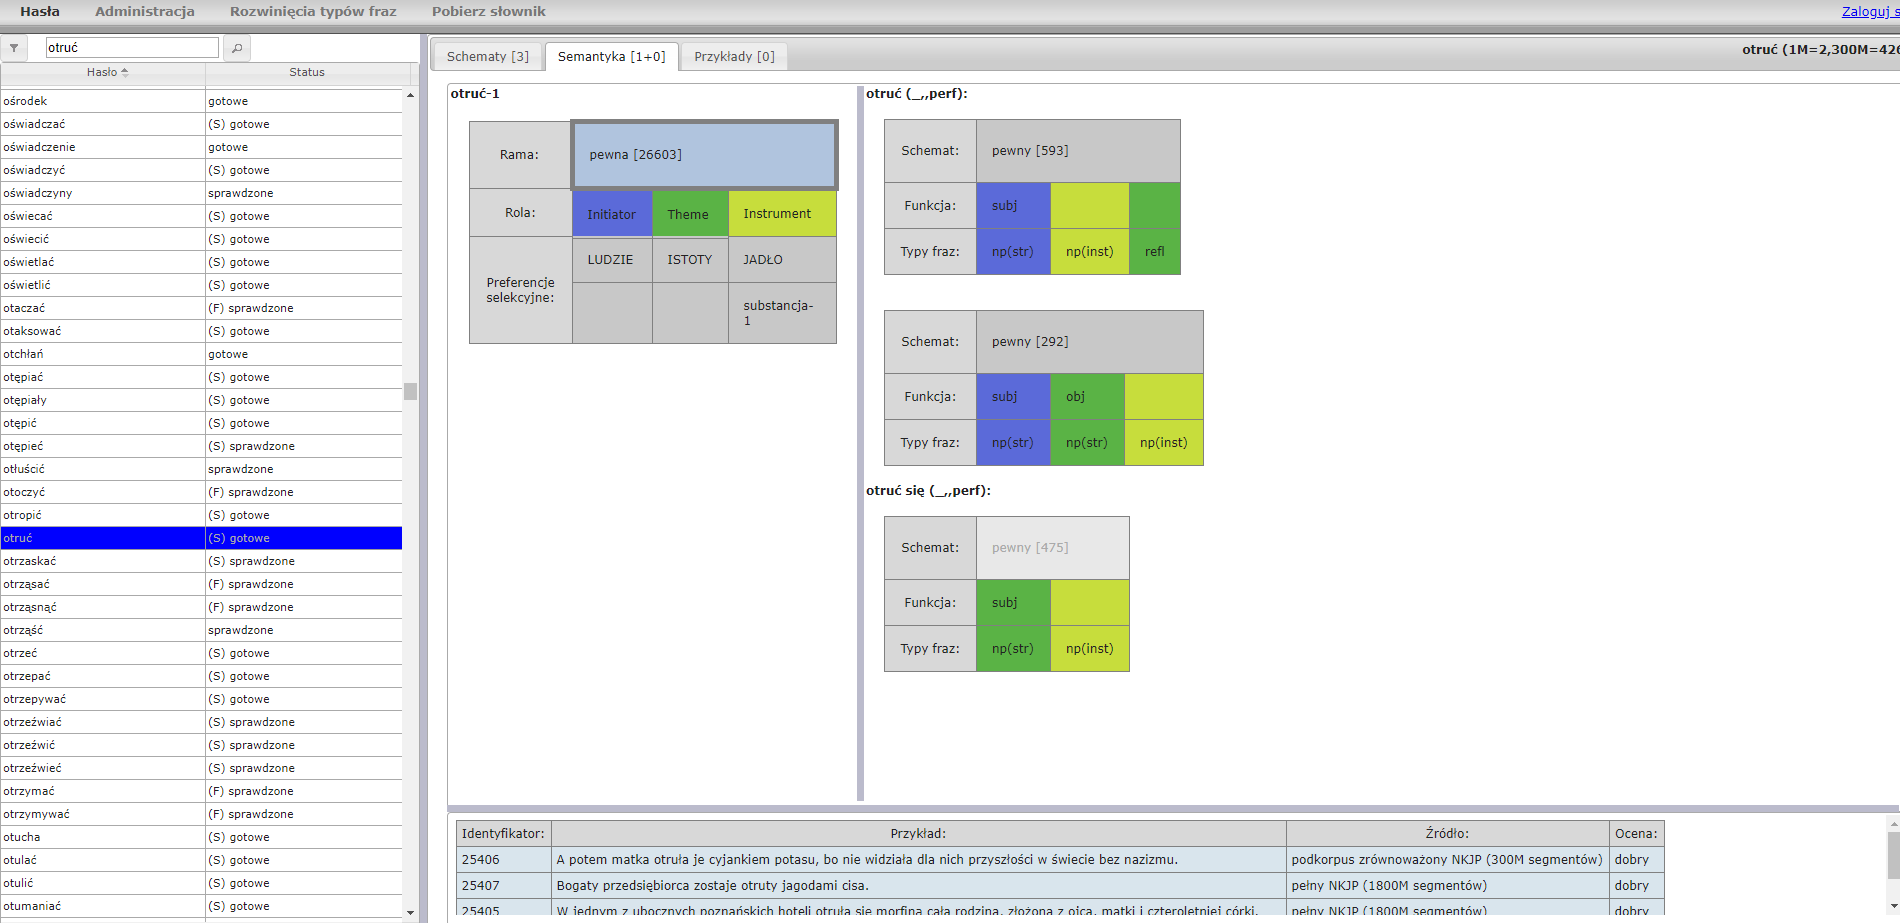
\includegraphics[width=\textwidth]{figures/grabowski-img001.png}
\caption{\label{fig:grabowski:1}. The verb otruć ‘to poison’ in Walenty (retrieved from: \url{http://walenty.clarin-pl.eu})}
\end{figure}

Although \textit{Walenty} is similar to Pattern Grammar in that it presents syntactic environments of lexical items, it does not allow the researcher to browse through larger lexico-grammatical patterns (e.g. verbs, nouns or adjectives and the words or syntagmatic frames that follow or precede the words) or to classify the slot-fillers in those patterns into specific meaning or functional groups, which is precisely what the Pattern Grammar approach does. For example, the so-called ‘introductory \textit{it}’ pattern followed by a link-verb, adjective and to-infinitive clause (\textbf{\textit{it}} \textbf{v-link} \textbf{{\ADJ}} \textbf{\textit{to}}\textbf{{}-inf})\footnote{The example is available at: \url{https://grammar.collinsdictionary.com/grammar-pattern/it-v-link-adj-to-inf_1}} reveals a number of meaning groups for adjectives filling in the pattern (\figref{fig:grabowski:2}) as well as specific examples of their use (\figref{fig:grabowski:3}).

  
\begin{figure}
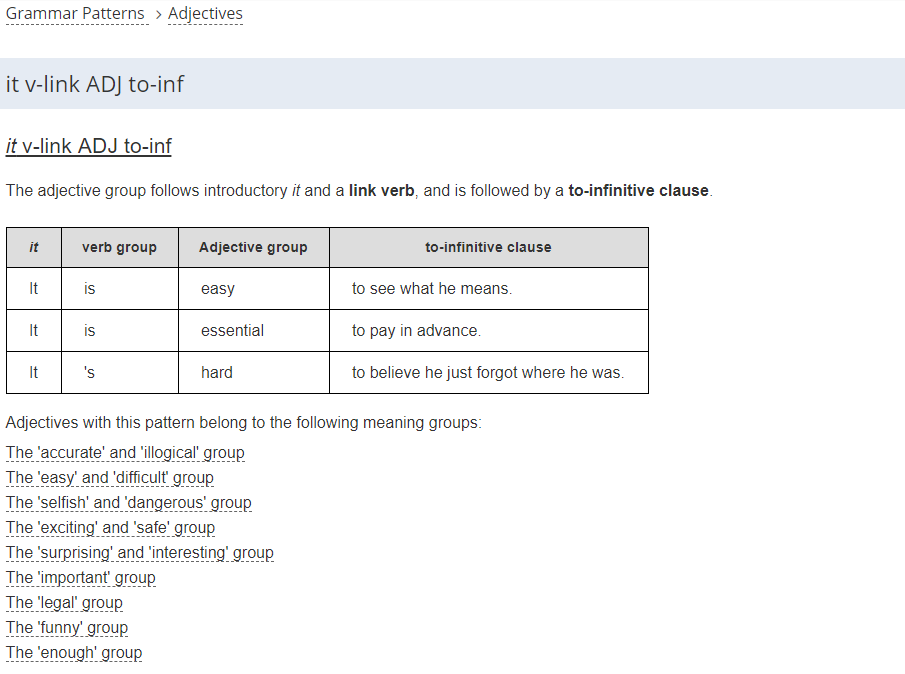
\includegraphics[width=\textwidth]{figures/grabowski-img002.png}
 \caption{\label{fig:grabowski:2}. The pattern ‘it v-link {\ADJ} to-inf’}
\end{figure}

\begin{figure}
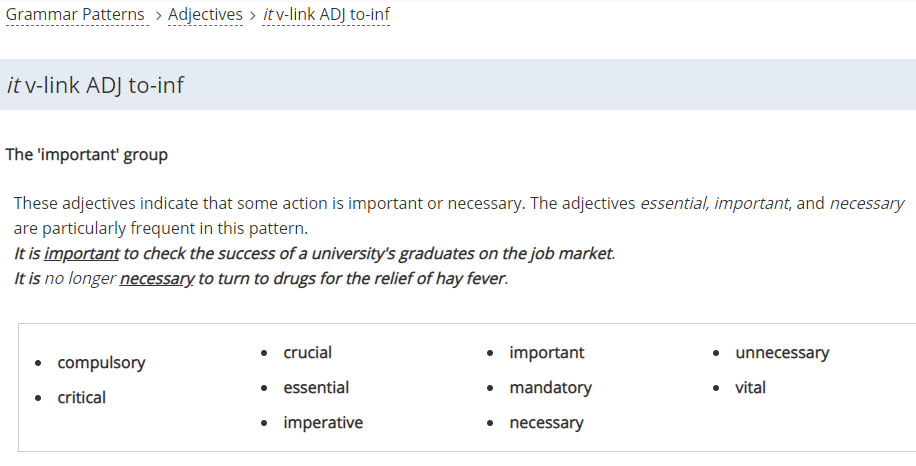
\includegraphics[width=\textwidth]{figures/grabowski-img003.png}
 \caption{\label{fig:grabowski:3}. The pattern ‘it v-link {\ADJ} to-inf’ filled with adjectives conveying the sense of importance.}
 \end{figure}

As can be seen in \figref{fig:grabowski:3}, the sense of importance (or attitudinal stance) of the following proposition is conveyed by the entire grammar pattern \textbf{\textit{it}} \textbf{v-link} \textbf{{\ADJ}} \textbf{\textit{to}}\textbf{{}-inf} rather than by individual adjectives filling in the pattern. Consequently, Pattern Grammar offers an inventory of lexico-grammatical constructions which constitute pairings of form with semantic or discoursal function.\footnote{In practice, identification of GPs is possible by analyzing concordance lines, which later involves grouping the patterns into notional categories (e.g. topical or functional ones) on the basis of different types of meanings conveyed in contexts. Although individual words can help in determination of those groupings, a qualitative analysis of a wider context of their occurrence is necessary to form appropriate groups and thus identify the patterns (\citealt{HunstonFrancis2000}: 162).} Such a resource describing lexico-grammatical patterns extracted from corpora in a bottom-up fashion has not been developed for the Polish language so far. 

The main goal of this study is therefore to explore whether GPs may be employed as a useful exploratory tool for cross-linguistic studies. In other words, we aim to identify and describe lexico-grammatical patterns that emerge from the English-to-Polish translations -- extracted from Paralela corpus \citep{Pęzik2016} -- of a pre-selected English GP performing specific discoursal functions. More precisely, we will focus on one English ‘introductory it’ pattern with \textit{to}{}-clause complementation (\textbf{\textit{it} }\textit{v-link}\textbf{ \textbf{{\ADJ}} \textbf{to-inf}}), which will constitute the starting point for our analysis.\footnote{Both patterns were studied by \citet{Groom2005} in terms of their variability across different academic registers.} However, the \textit{tertium comparationis} are the functional categories or discoursal functions (necessity, importance, obviousness etc.) contingent on individual words filling in the patterns or, in other words, worked out on the basis of intuitive understandings of words in the English GPs. This will allow us to investigate whether we may find corresponding generalizable lexico-grammatical patterns in Polish that perform the same discoursal functions as the English GP under scrutiny. The underlying assumption is that in theory the Polish translations should convey the same information as their English source texts. We will also attempt to verify whether GPs are useful as a discovery tool for detecting translation patterns. We believe that a study like this one may pave the way to a wider application of the Pattern Grammar approach for the description of languages other than English (in this case, Polish) and/or for cross-linguistic comparisons or translation-oriented research, which have not been attempted hitherto. 

The chapter is structured as follows. In \sectref{sec:grabowski:2}, the research material (i.e. the study corpus), units of analysis and methodology will be described. Next, we describe and discuss the empirical results exemplifying translation patterns emerging from textual realizations of GPs in the sample of English source-texts and their Polish translations. The concluding section discusses the study limitations and offers suggestions on how this research may be developed further in the future.

\section{Methodology}\label{sec:grabowski:2}
\subsection{Research material}

For the purposes of the current study, we will use the English-Polish parallel corpus \textit{Paralela} \citep{Pęzik2016}.\footnote{Available at: \url{http://paralela.clarin-pl.eu}.} The parallel corpus under scrutiny includes a little more than 262 million word tokens in 10,877,000 translation segments from various text types and genres, including written, spoken and to-be spoken texts, e.g. legal documents from various European Union institutions (legislation, transcripts of proceedings of the European Parliament etc.), press releases, medical texts, film subtitles, popular science texts, literary classics, transcripts of European Parliament proceedings etc. As a rule, a parallel corpus contains source texts aligned with their translations in the target language. In this study, we will analyze a pre-selected GP (‘\textit{it} v-link {\ADJ} \textit{to}{}-inf’) found in a single genre of English source texts, namely European Parliament proceedings (henceforth EPP), and we will try to align its textual realizations with their Polish equivalents as found in translation segments in the corresponding Polish sub-corpus (with more than 13 million word tokens in almost 700,000 translation segments)\footnote{The transcripts were originally extracted from Europarl corpus \citep{Koehn2005} and included in Paralela. The debates were recorded on 11--12th and 23rd October 2006, and translated from English into Polish.} Then, we will attempt to quantitatively and qualitatively analyze the target language equivalents and see whether any regular patterns, i.e. lexico-syntactic associations similar to GPs, emerge from the Polish language data.

\subsection{Units of analysis}

At least in theory, parallel corpora include texts (originals and translations) that express the same meanings and perform the same discoursal functions, which allows one to search for correspondences between linguistic items in source and target texts (\citealt{Johansson2007}: 9, cited in \citealt{Marco2019}: 43). As mentioned earlier, in this study we will focus on a pre-selected GP, which means that the lexical items under scrutiny will not be extracted from texts in a bottom-up approach. This is mainly because we do not have access to full texts collected in \textit{Paralela}. Hence, the use of the study corpora will be limited to the analysis of bilingual concordances illustrating particular translation patterns, i.e. frequency and distribution of the Polish equivalents of the English GP, which provide a starting point for our investigation. 

We will capitalize on the results of the study conducted by \citet{Groom2005}, who analyzed, among others, two GPs, namely \textbf{\textit{it} }\textbf{v-link \textbf{{\ADJ}} \textbf{that}} and \textbf{\textit{it} }\textbf{v-link \textbf{{\ADJ}} \textbf{to-}}\textbf{inf}. \citet[259--260]{Groom2005} noticed that adjectives which convey the meaning (i.e. sense) that can be generalized as “validity” (e.g. \textit{clear, inconceivable, obvious}) tend to fall into the pattern \textbf{\textit{it} }\textbf{v-link} \textbf{\textit{{\ADJ}} \textbf{that}} while the adjectives conveying the sense of “difficulty” (e.g. \textit{difficult, easy, hard}) tend to fall into the pattern \textbf{\textit{it} }\textbf{v-link \textbf{{\ADJ}} \textbf{to-}}\textbf{inf}\footnote{However, \citet{Groom2005} found that distributions and more fine-grained rhetorical functions of the adjectives in those grammar patterns vary across corpora representing different language varieties.}. Also, it was found that depending on the pattern, one and the same word (e.g. the adjective \textit{possible}) may convey different senses, that is either “difficulty” or “validity” \citep[259]{Groom2005}. In summary, the findings of the study conducted by \citet{Groom2005} provide strong evidence of the relationship between particular sense conveyed by particular words and the structural patterns in which those words tend to occur.

We will search for a single pre-selected pattern using the SlopeQ query syntax implemented in \textit{Paralela} as well as morphosyntactic tags (e.g. \texttt{<tag=j.*>} stands for adjectives). Thus, the pattern \textbf{\textit{it} }\textbf{v-link \textbf{{\ADJ}} \textbf{to-}}\textbf{inf} will be searched for using the following query:

\begin{quote}
\texttt{it <tag=v.*> <tag=j.*> to}\\
(34,047 occurrences in Paralela; 3,067 occurrences in EPP).
\end{quote}

In view of a high number of occurrences, it is necessary to filter out the results to facilitate the qualitative analysis of concordance lines. To this end, we will apply systematic sampling by recording translation pairs of every 30\textsuperscript{th} concordance. This means that we will ultimately focus on a sample of 100 translation pairs (i.e. bilingual concordances illustrating Polish translations of specific textual realizations of the English GP) extracted from the EPP sub-corpus of \textit{Paralela}.

\subsection{Research questions and hypotheses}

The main problem addressed in this study concerns whether the corresponding items (translation equivalents) found in target texts can also be described in terms of recurrent lexico-syntactic associations similar to the GP identified in the English source texts. Hence, in this exploratory paper we aim to provide answers to the following research questions:

\begin{description}
\item[RQ1:] What are the Polish equivalents of the English source-language multi-word items emerging from GPs?
\item[RQ2:] Can the Polish equivalents be generalized into a more abstract set of lexico-grammatical patterns similar to GPs?
\item[RQ3:] Can the Pattern Grammar approach be used for a description of Polish?
\item[RQ4:] Can GPs be applied as a unit of analysis in cross-linguistic contexts?
\end{description}

\subsection{Research questions and hypotheses}

This study will be conducted in a number of stages. First, we will preselect one GP (described earlier) and develop an inventory of their textual realizations in English source-texts, i.e. in the EPP sub-corpus of \textit{Paralela}. Then, we will generalize the results by means of grouping overlapping textual realizations into a list of n-grams performing specific discourse functions. After identification of the Polish equivalent, or translation variant (be it a single-word or a multi-word unit), we will investigate whether the observed patterns of Polish translations can be generalized to a more abstract phraseological, syntagmatic or lexico-grammatical units, similar to GPs.

\section{Preliminary results: Grammar patterns in contrast}

In this exploratory study, we used the GP \textbf{\textit{it} }\textbf{v-link \textbf{{\ADJ}} \textbf{to-}}\textbf{inf} as a unit of analysis and a tool for discovering potential translation patterns. All in all, the said GP occurred in the EPP sub-corpus of Paralela 3,067 times. In order to limit the amount of data for manual analysis of bilingual concordances, we used systematic sampling and selected every 30\textsuperscript{th} concordance, which resulted in the set of 100 English-Polish translation segments to be analyzed. Depending on the adjectives filing in the slot, we used the procedure put forward by \citet{Groom2005} and -- by conducting manual analysis of English source-text fragments -- we classified the textual variants of the GP found in the sample into semantic/functional categories (discoursal functions) corresponding to the senses conveyed by the adjectives. This way, the linguistic data were classified into the following categories: \textsc{importance}, \textsc{validity}, \textsc{desirability} and \textsc{difficulty}.

First, we present the results of the analysis of the textual instantiations of the GP \textbf{\textit{it}} \textbf{v-link \textbf{{\ADJ}} \textbf{to-}}\textbf{inf} as filled with adjectives conveying the sense of ‘difficulty’ in the English-original texts in the EPP sub-corpus (8 occurrences) and its equivalents in the Polish translations.


\begin{table}
\begin{tabularx}{\textwidth}{QQQ}
\lsptoprule
Textual realizations in the English-original & Polish equivalents & Generalized pattern of Polish translations \\
\midrule
\textit{it is} \textbf{\textit{difficult}} \textit{to} (5)  &  \textbf{\textit{trudno}} \textit{jest} (5) & {\ADV} v-link v-inf\\
\textit{it is} \textbf{\textit{hard}} \textit{to} (2)  &  \textbf{\textit{trudno}}\textit{, aby} (1)  & {\ADV}, \textit{aby}\\
                                                       &  \textbf{\textit{trudno}} (1) & {\ADV} v-inf\\
\textit{it is} \textbf{\textit{easier}} \textit{to} (1)  &  \textbf{\textit{łatwiej}} (1) & {\ADV} v{}-inf\\
\lspbottomrule
\end{tabularx}
\caption{Textual realizations of the GP \textbf{\textit{it} \textbf{v-link} \textbf{{\ADJ}} \textbf{to-inf}} in English source-texts and their Polish translations: Discoursal function of \textsc{difficulty}\label{tab:grabowski:1}}
\end{table}

The findings (\tabref{tab:grabowski:1}) show that in the sample under scrutiny there are three different instantiations of the English GP ‘\textit{it} v-link {\ADJ} \textit{to}{}-inf’ when filled with adjectives conveying the sense of ‘difficulty’, namely \textit{it is difficult to}, \textit{it is hard to} and \textit{it is easier to}, with the total frequency of 8. Those multi-word items have the following Polish equivalents in Paralela corpus, such as \textit{trudno jest} (used 5 times as an equivalent of \textit{it is difficult to}), \textit{trudno, aby} and \textit{trudno} (used 1 each as equivalents of \textit{it is hard to}) and \textit{łatwiej} (used once as an equivalent of \textit{it is easier to}). Apart from insights into certain translational choices, it has been possible to reconstruct abstract lexico-grammatical patterns (or syntagmatic frames) based on the Polish equivalents and conveying the sense of difficulty with respect to the following proposition, e.g. ‘{\ADV} v-link v-inf’ (\textit{trudno jest}) or ‘{\ADV} v-inf’, both followed by a verb in infinitive form (\textit{trudno jest udowodnić ‘}it is difficult to prove’\textit{, trudno uwierzyć} ‘it is difficult to believe’) or ‘{\ADV}, \textit{aby}’ (\textit{trudno, aby} etc.) followed by a complement clause, e.g.:,

\ea
\ea \textbf{\textit{It} \textbf{is} \textbf{hard} \textbf{to}} \textit{believe when reading it.}\\
\textbf{\textit{Trudno} }\textit{uwierzyć w te słowa, kiedy się je czyta.} [EVOeRj]
\ex \textit{This is because} \textbf{\textit{it} \textbf{is} \textbf{difficult} \textbf{to}} \textit{prove that the service rendered was of poor quality.}\\
\textit{Dzieje się tak dlatego, że} \textbf{\textit{trudno} \textbf{jest}} \textit{udowodnić, że świadczone usługi były złej jakości.} [qoavWA]
\ex \textit{Simplification of the common agricultural policy is a beautiful idea, and} \textbf{\textit{it} \textbf{is} \textbf{hard} \textbf{to}} \textit{imagine that someone would oppose it.}\\ 
\textit{Uproszczenie wspólnej polityki rolnej to piękna idea i} \textbf{\textit{trudno,} \textbf{aby}} \textit{ktoś był jej przeciwny.} [ea2Eoq]
\z
\z

As can be seen, the English GP ‘\textit{it} v-link {\ADJ} \textit{to}{}-inf’, when filled by adjectives conveying the sense of ‘difficulty’, corresponds to a set of Polish syntagmatic patterns, such as ‘{\ADV}, \textit{aby}\,+\,complement clause’, ‘{\ADV} v-link v-infinitive’ or ‘{\ADV} v-infinitive’.

The following example under scrutiny refers to the GP ‘\textit{it} v-link {\ADJ} \textit{to}{}-inf’ as filled with adjectives (\textit{possible, clear, impossible, true}) conveying the sense of ‘validity’ in the English-source texts (\tabref{tab:grabowski:2}).


\begin{table}
\begin{tabularx}{\textwidth}{QQQ}
\lsptoprule
Textual realizations in the English-original & Polish equivalents & Generalized pattern of Polish translations\\\midrule
\textit{(will) it be} \textbf{\textit{possible}} \textit{to} (1)  &  \textbf{\textit{możliwe}} \textit{(będzie)} (1) & {\ADJ} v-link\\

\midrule
\textit{it is} \textbf{\textit{clear}} \textit{to (us/me)} (2)  &  \textit{dla (nas)} \textbf{\textit{jasne}} \textit{jest, że} (1)  & {\ADJ} v-link, \textit{że} ‘that’\\
                                                                &  \textit{jest dla (mnie)} \textbf{\textit{jasne}}\textit{, że} (1) & v-link {\ADJ}, że ‘that’\\
\midrule
\textit{it is} \textbf{\textit{impossible}} \textit{to} (1)  &  \textbf{\textit{niemożliwością}} \textit{jest} (1) ‘impossibility is’ & \textsc{nn} v-link\\
                                                             &    \textit{nie można} (1) ‘ &  \textsc{neg}prt\,+\,\textsc{mod} v \\
\midrule
\textit{it is} \textbf{\textit{possible}} \textit{to} (4)  &  \textbf{\textit{możliwe}} \textit{jest} (2) ‘possible that’ &   {\ADJ} v-link   \\
                                                                    &      \textit{można} (1) ‘may/can’                             &     \textsc{mod}v v-inf    \\
                                                                    &       \textit{możliwość}\footnote{\textrm{(EN)}\textrm{ }\textrm{\textit{I would like to say that} }\textrm{\textbf{\textit{it} \textbf{is} \textbf{becoming} \textbf{clear}}}\textrm{ \textit{in this discussion that it is possible to have a 'two-speed' Europe.} }\textrm{(PL)}\textrm{ \textit{Chciałbym powiedzieć, że w tej dyskusji} }\textrm{\textbf{\textit{oczywista} \textbf{staje} \textbf{się} \textbf{możliwość}}}\textrm{ \textit{istnienia Europy "dwóch szybkości”.}} \textrm{[Drag45]}} (1) ‘possibility’     &     \textsc{transformation}\\
\midrule
\textit{it is} \textbf{\textit{true}} \textit{to} (1) say  &  \textbf{\textit{prawdą}} \textit{jest, że} (1) ‘truth is that’ & \textsc{nn} v-link, \textit{że} ‘that’\\
\lspbottomrule
\end{tabularx}
\caption{Textual realizations of the GP ‘it v-link ADJ to-inf’ in English source-texts and their Polish translations: discoursal function of \textsc{validity}\label{tab:grabowski:2}}
\end{table}

The findings show that there is more variety among Polish lexico-grammatical patterns that convey the sense of ‘validity’ in the Polish translations as compared with the sense of ‘difficulty’. The most frequent one (4 occurrences) is the pattern ‘{\ADJ} v-link’ (with positional variation) and ‘{\ADJ} v-link, \textit{że}’, which is realized with the following Polish equivalents, namely \textit{możliwe} (\textit{będzie}); \textit{możliwe jest;} (…) \textit{jasne jest, że}; \textit{jest} (…) \textit{jasne, że}. Other patterns are centred around nouns (‘{\NN}’, ‘{\NN} v-link’ and ‘{\NN} v-link, \textit{że}’), which include the following words and phrases: \textit{możliwość}, \textit{niemożliwością jest} and \textit{prawdą jest, że} respectively, e.g.:

\ea
 \textit{I would like to say that it is becoming clear in this discussion that} \textbf{\textit{it} \textbf{is} \textbf{possible} \textbf{to}} \textit{have a 'two-speed ' Europe.}\\
\textit{Chciałbym powiedzieć, że w tej dyskusji oczywista staje się} \textbf{\textit{możliwość}} \textit{istnienia Europy "dwóch szybkości}\footnote{\textrm{The phrase} \textrm{\textit{Europa dwóch szybkości}} \textrm{‘two-speed Europe’ has not been adopted in the Polish press discourse. Instead, the phrase} \textrm{\textit{Europa dwóch prędkości}} \textrm{has become commonly used.} }\textit{”.}[Drag45]
\z

There are also two patterns centred on the modal verb \textit{można} ‘can/may’ (‘{\MOD}v’, ‘{\NEG} {\PRT} {\MOD}v’), namely \textit{można} and \textit{nie można}, followed by the infinitive form of the verb, e.g.:

\ea
 (…) \textit{but the one thing I have learned is that} \textbf{\textit{it} \textbf{is} \textbf{impossible} \textbf{to}} \textit{book a ticket on the Eurostar when you are travelling}.\\
 (…) \textit{lecz nauczyłem się jednego, a mianowicie, że} \textbf{\textit{nie} \textbf{można}} \textit{zarezerwować biletu na pociąg}. [BNzRG4]
\z

A large group of multi-word items in the English originals conveys a sense of ‘importance’ (e.g. \textit{it is important to, it is crucial to, it is essential that}) and there is a high variety among their Polish equivalents, which can be grouped into a number of lexico-grammatical patterns. The most prominent ones include the pattern ‘{\ADJ} v-link’ and ‘{\ADJ} v-link, \textit{aby/by’} (e.g. \textit{istotne jest}; \textit{ważne jest, aby}; \textit{niezbędne jest; konieczne jest}), with adjectives occasionally modified by adverbs (e.g. \textit{bardzo ważne jest}, \textit{niezwykle istotne jest}). It is particularly noticeable that the pattern ‘{\ADJ} v-link’ is followed by a verbal noun functioning as a direct object, while the pattern ‘{\ADJ} v-link, \textit{aby/}by’ or ‘{\ADJ}, \textit{by}’) is followed by the verb in the infinitive form, e.g.:

\ea
\ea \textit{Finally, I would like to stress that} \textbf{\textit{it} \textbf{is} \textbf{important} \textbf{to}} \textit{have full transparency regarding the founding of the initiative and sources of financial support for the organisers.}\\
\textit{Wreszcie, pragnę podkreślić, że} \textbf{\textit{ważne} \textbf{jest}} \textit{zapewnienie pełnej przejrzystości w odniesieniu do finansowania inicjatywy oraz źródeł wsparcia finansowego dla jej organizatorów} [RDwmvo]
\ex \textbf{\textit{It} \textbf{is} \textbf{important} \textbf{to}} \textit{overcome the current problems that characterise the sector: the lack of competition, the regulatory over-dependence on ratings, and the low reliability of notes.} \\
\textbf{\textit{Ważne} \textbf{jest,} \textbf{aby}} \textit{rozwiązać problemy, które obecnie spotyka się w tej branży, a mianowicie przesadne zawierzanie ratingom i małą wiarygodność ocen.} [APaN8r]
\z
\z

Other frequent patterns include ‘{\MOD}v v-inf’ (\textit{trzeba, musimy/musi, należy} followed by verbs in the infinitive form) or ‘{\NN} {\ADJ} v-link’ (e.g. \textit{sprawą podstawową jest}; \textit{ważną rzeczą jest/są}) or ‘{\glossV} {\ADJ} {\NN}’ (e.g. \textit{ma fundamentalne znaczenie}), cf. \tabref{tab:grabowski:3} below.

\begin{table}\footnotesize
\begin{tabularx}{\textwidth}{lQl}
\lsptoprule
Original & Polish equivalents & GP in Polish trans. \\
\midrule
\textit{it is} \textbf{\textit{important} }\textit{to} (1)  &  \textbf{\textit{ważne}} \textit{jest, aby} (1) & {\ADJ} v-link, \textit{aby}\\

\midrule
\textit{it is} \textbf{\textit{crucial}} \textit{to} (2)  &  \textbf{\textit{istotne}} \textit{jest} (1)   & {\ADJ} v-link\\
                                                          &  \textbf{\textit{kluczowe}} \textit{znaczenie ma} (1) & {\ADJ} {\NN} {\glossV}\\

\midrule
\textit{it is} \textbf{\textit{essential}} \textit{to} (10) &  \textbf{\textit{konieczne} }\textit{jest} (2)                             &  {\ADJ} v-link            \\
                                                             &  \textbf{\textit{kluczowe}} \textit{znaczenie ma} (2)                      &  {\ADJ} {\NN} {\glossV}              \\
                                                             &  \textbf{\textit{niezbędne}} \textit{jest} (2)                             &  {\ADJ} v-link            \\
                                                             &  \textit{trzeba} (1)                                                       &  {\MOD}v v-inf            \\
                                                             &  \textit{ma} \textbf{\textit{istotne} \textbf{znaczenie}} (1)              &  {\glossV} {\ADJ} {\NN}              \\
                                                             &  \textbf{\textit{niezwykle}} \textbf{\textit{istotne}} \textit{jest} (1)   &  ({\ADV}) {\ADJ} v-link      \\
                                                             &  \textit{należy} (1)                                                       &  {\MOD}v v-inf            \\

\midrule
\mbox{\textit{it is} \textbf{\textit{fundamental}} \textit{to} (1)}  &  \textit{ma} \textbf{\textit{fundamentalne} \textbf{znaczenie}} (1) & {\glossV} {\ADJ} {\NN}\\

\midrule
\textit{it is} \textbf{\textit{imperative}} \textit{to} (1)  &  \textbf{\textit{bardzo} \textbf{ważne}} \textit{jest} (1) & ({\ADV}) {\ADJ} v-link\\

\midrule
\textit{it is} \textbf{\textit{important}} \textit{to} (24)  &  \textit{należy} (6)                                                 & {\MOD}v v-inf                      \\
                                                             &  \textbf{\textit{ważne}} \textit{jest} (6)                           & {\ADJ} v-link                      \\
                                                             &  \textit{musimy} (1)                                                 & {\MOD}v v-inf                      \\
                                                             &  \textit{należy} \textbf{\textit{koniecznie}} (3)                    & {\MOD}v {\ADV} v-inf                  \\
                                                             &  \textbf{\textit{ważne}} \textit{jest, aby} (2)                      & {\ADJ} v-link, \textit{aby}        \\
                                                             &  \textit{trzeba} (2)                                                 & {\MOD}v v-inf                      \\
                                                             &  \textbf{\textit{bardzo} \textbf{ważne}} \textit{jest} (1)           & {\ADJ} v-link                      \\
                                                             &  \textbf{\textit{konieczne}} \textit{jest} (1)                       & {\ADJ} v-link                      \\
                                                             &  \textbf{\textit{ważną} \textbf{rzeczą}} \textit{jest/są} (1)        & {\ADJ} N v-link                    \\
                                                             &  \textbf{\textit{ważne}}\textit{, by} (1)                            & {\ADJ}, \textit{by}                \\
                                                             &  \textbf{\textit{najważniejsze}} \textit{jest} (1)                   & {\ADJ} v-link                    \\
\midrule
\textit{it is} \textbf{\textit{necessary}} \textit{to} (15)  &  \textit{należy} (4)  & {\MOD}v v-inf\\
                                                             &    \textbf{\textit{konieczne}} \textit{jest} (3) & {\ADJ} v-link\\
                                                             &    \textit{wymaga}\footnote{{(EN)} {\textit{There is also a need to measure quality of life in societies, because in order to ensure and sustain quality of life,} }{\textbf{\textit{it} \textbf{is} \textbf{necessary} \textbf{to}}}{ \textit{take into account important, consensual factors such as health, education, culture, employment, housing, environmental conditions etc.}} {(PL)} {\textit{Istnieje także potrzeba pomiaru jakości życia w społeczeństwach, ponieważ osiągnięcie oraz utrzymanie odpowiedniej jakości życia} }{\textbf{\textit{wymaga}}}{ \textit{(‘requires’) uwzględnienia istotnych i jednomyślnie uznanych czynników, takich jak zdrowie, edukacja, kultura, zatrudnienie oraz warunki mieszkaniowe, środowiskowe itp.}} {[6nv4bb]}} (2)                                & {\glossV}\\
                                                             &    \textit{trzeba} (2) & {\MOD}v v-inf\\
                                                             &    \textit{trzeba} \textbf{\textit{koniecznie}} (1) & {\MOD}v {\ADV} v-inf\\
                                                             &    \textit{rzeczą} \textbf{\textit{konieczną}} \textit{jest} (1)     & {\NN} {\ADJ} v-link   \\
                                                             &    \textit{musi} (1) & {\MOD}v v-inf\\

\midrule
\textit{it seems} \textbf{\textit{fundamental}} \textit{to} (1) me  &  \textbf{\textit{sprawą} \textbf{podstawową}} \textit{jest} (1) & {\NN} {\ADJ} v-link\\

\midrule
\textit{it was} \textbf{\textit{essential}} \textit{to} (1)  &  \textit{było (jest)} \textbf{\textit{niezwykle} \textbf{istotne}} (1) & v-link {\ADV} {\ADJ} \\
\lspbottomrule
\end{tabularx}
\caption{Textual realizations of the GP ‘it v-link {\ADJ} to-inf’ in English source-texts and their Polish translations: discoursal function of \textsc{importance}\label{tab:grabowski:3}}
\end{table}

\begin{table}\footnotesize
\begin{tabularx}{\textwidth}{QQQ}
\lsptoprule
Textual realizations in the English-original & Polish equivalents & Generalized pattern in Polish translations \\\midrule
\textit{it is} \textbf{\textit{necessary}} \textit{to} (1)  &  \textbf{\textit{konieczne}} \textit{jest} (1) & {\ADJ} v-link\\
\textit{it is} \textbf{\textit{advisable}} \textit{to} (1)  &  \textsc{omission}\footnote{\textrm{(EN)} \textrm{\textit{We shall check what you have said, and you can rest assured that, within the context of measures available to the Council and the work on implementing the Pact on Immigration and Asylum,} }\textrm{\textit{we shall look once more at}}\textrm{ \textit{whether} }\textrm{\textbf{\textit{it} \textbf{is} \textbf{advisable} \textbf{to}}}\textrm{ }\textrm{\textit{reinforce this point}}\textrm{ \textit{within the framework of the Schengen area.}} \textrm{(PL)} \textrm{\textit{Sprawdzimy to, o czym pan mówił, i może pan mieć pewność, że w kontekście środków, jakimi dysponuje Rada, oraz prac nad wdrożeniem paktu o imigracji i azylu,} }\textrm{\textit{ponownie przemyślimy}}\textrm{ }\textrm{\textit{kwestię udoskonalenia tego elementu}}\textrm{ \textit{w ramach strefy Schengen.}} \textrm{[AP01Ae]}} (1) & \textsc{omission}\\
\textit{it is} \textbf{\textit{appropriate}} \textit{to} (1)  &  \textbf{\textit{warto}} (1) ‘it is worth’ & {\MOD}v v-inf\\
\textit{it is} \textbf{\textit{better}} \textit{to} (1)  &  \textbf{\textit{lepiej}} (1) ‘better’ & {\ADV} {\glossV}\\
\textit{it is} \textbf{\textit{fair}} \textit{to} (1) (\textit{say that…})  &  \textbf{\textit{uczciwie}} (1) ‘fairly’ & \textsc{transformation}\footnote{\textrm{(PL) (…)} \textrm{\textit{będzie uczciwie, jeżeli powiem, że (…)}} \textrm{[rBwJxM]}}\\
\textit{it is} \textbf{\textit{good}} \textit{to} (1) know  &  \textbf{\textit{dobrze}} \textit{jest} (1) & {\ADV} v-link\\
\textit{it is} \textbf{\textit{inappropriate}} \textit{to} (1)  &  \textit{jest} \textbf{\textit{niestosowne}} (1) & v-link {\ADJ}\\
\textit{it is} \textbf{\textit{irresponsible}} \textit{to} (1)  &  \textbf{\textit{nieodpowiedzialne}} \textit{jest} (1) & {\ADJ} v-link\\
\textit{it is} \textbf{\textit{nice}} \textit{to} (1) (\textit{have you with us})  &  \textit{Cieszymy się, że} (1) \textit{jest Pan tu z nami} ‘we are happy to have you here with us’ & \textsc{fixed formula}\\
\textit{it is} \textbf{\textit{pointless}} \textit{to} (1)  &  \textit{nie ma sensu} (1) & {\NEG}prt {\glossV} {\NN}\\
\textit{it is} \textbf{\textit{profitable}} \textit{to} (1)  &  \textit{przynosi zysk}  & {\glossV} {\NN}\\
\textit{it is} \textbf{\textit{right}} \textit{to} (3)  &  \textit{należy} (1) \textit{jest} \textbf{\textit{słuszne}} (1) \textbf{\textit{słuszne}} \textit{jest} (1) & {\MOD}v v-inf v-link {\ADJ} {\ADJ} v-link\\
\textit{it is} \textbf{\textit{sensible}} \textit{to} (1)  &  \textit{(jest)} \textbf{\textit{rozsądne}} (1) & v-link {\ADJ}\\
\textit{it is} \textbf{\textit{unacceptable}} \textit{to} (1)  &  \textit{nie do przyjęcia jest} (1) & {\NEG}prt {\PREP} {\NN} v-link\\
\textit{it is} \textbf{\textit{uplifting}} \textit{to} (1)  &  \textit{świadomość} (…) \textit{podnosi na duchu} (1) ‘awareness of (…) raises sb’s spirits' & \textsc{transformation}\\
\textit{it is} \textbf{\textit{worthwhile}} \textit{to} (1)  &  \textbf{\textit{warto}} (1) & {\MOD} v v-inf\\
\textit{it was} \textbf{\textit{agreeable}} \textit{to} (1)  &  \textit{miło było} (1) ‘(it) was nice to’ & {\ADV} v-link v-inf\\
\lspbottomrule
\end{tabularx}
\caption{Textual realizations of the GP ‘it v-link {\ADJ} to-inf’ in English source-texts and their Polish translations: Discoursal function of \textsc{desirability}.\label{tab:grabowski:4}}
\end{table}

Finally, similar correspondences can be observed in the case of structures conveying the sense of ‘desirability’ in the English originals and their Polish equivalents (\tabref{tab:grabowski:4}). The most frequent patterns -- with positional variation due to free word order -- in the Polish translations were found to be ‘{\ADJ} v-link’ (e.g. \textit{konieczne jest, jest niestosowne, nieodpowiedzialne jest, słuszne jest}), ‘{\ADV} v-link’ (e.g. \textit{dobrze jest}), ‘{\MOD}v v-inf’ (e.g. \textit{warto, należy}). The comparison of certain GPs provides interesting insights into cross-linguistic correspondences on the syntactic level. For example, the English pattern ‘\textit{it} v-link {\ADJ} v-inf’ may correspond, among others, to the Polish GP ‘{\MOD}v v-inf’, where the position of direct and indirect object with respect to the patterns under scrutiny changes, e.g. 

\ea \textbf{\textit{It} \textbf{is} \textbf{essential} \textbf{to}} \textit{give people} [Indirect object] \textit{access} [Direct object] \textit{to healthcare, drinking water and sanitation.} 
\ex\textit{Ludziom} [Indirect object] \textbf{\textit{należy}} \textit{zapewnić dostęp} [Direct object]\footnote{\textrm{Lit. ‘people should be given access’}} \textit{do opieki zdrowotnej, wody pitnej i kanalizacji.} [DrZG0o]
\z

We also identified ready-made formulas corresponding to specific speech acts, (e.g. the polite phrase used after a greeting \textit{Cieszymy się, że jest Pan tu z name} versus \textit{it is nice to have you with us}) or transformations resulting from stylistic changes in the translation as compared to the original. Both fixed formulas and transformations do not fall into GPs that we attempted to identify among the Polish equivalents.

\section{Discussion and conclusions}

The findings of our exploratory study indicate that the Pattern Grammar approach holds unexplored potential for cross-linguistic research, of both text-ori\-ent\-ed and system-oriented kinds. The approach showcased in our chapter used a set of GPs as a starting point to identify recurrent English multi-word items with specific meanings (senses) and discoursal functions, which were then aligned with their Polish equivalents. We obtained further empirical evidence against a widely held misconception about translation whereby one has to translate a given fixed phrase from L1 (English) into a corresponding fixed phrase in L2 (Polish). Using this methodology, we were able to obtain a set of lexico-grammatical frames emerging from the English-to-Polish translation patterns in the corpus under scrutiny (EPP). As well as yielding insights into language in use in English-to-Polish translation in the EPP corpus, our methodology revealed a number of novel and valuable cross-linguistic correspondences between formulaic structures in English and Polish. In the future, it is necessary to verify to what extent those Polish lexico-grammatical patterns can be generalized to other text types or genres (if we adopt a textual perspective focusing on language in use), and to the Polish language system (if we adopt a cross-linguistic systemic perspective). Nevertheless, our preliminary results are certainly encouraging. 

The findings of the current study also show that the Pattern Grammar approach, a linear and less formalized corpus-based grammatical description of how words are used in texts (i.e. with what phrases and clauses) (\citealt{HunstonFrancis2000}), holds unexplored potential not only for cross-linguistic studies, but also for the description of recurrent lexico-syntactic constructions found in other languages, such as Polish. Clearly, such a research agenda needs to be pursued with caution in view of the many typological differences between English and Polish (cf. \citealt{FisiakEtAl1978, WillimMańczak-Wohlfeld1997}). In practice, what this means is that a “Polish version” of Pattern Grammar will need to be mindful of formal descriptions of Polish, and that we should expect to find non-formally corresponding grammar patterns that convey the same meanings or discourse functions in English and Polish, as was the case with the English GP ‘\textit{it} v-link {\ADJ} \textit{to}{}-inf’ and the lexico-syntactic patterns that emerged from the Polish translations, rather than exact equivalents for each given English GP. Indeed, we may find that there are one-to-one, one-to-many, many-to-many and many-to-one relationships between GPs conveying the same meaning or discourse function in English and Polish. Since adjective complementation patterns have received considerable attention (e.g. \citealt{SuHunston2019}), it would be useful for future research to conduct analyses that involve other patterns (e.g. \textit{there} v-link \textit{sth/anything/nothing} {\ADJ} \textit{about/in} NP). Since this study concerns translation, it would be also interesting for future research to examine whether the observed translation patterns are triggered by English (due to interference), and if so then to what extent, or whether they are natural and equally formulaic in native Polish texts. Since this preliminary study is exploratory in nature, no frequency threshold was set to verify when an equivalent is regarded as a pattern; however, setting such a threshold will be essential in the future. 

Finally, Pattern Grammar-based descriptions of Polish may also feed into the future development of more comprehensive lexicographic resources, the so-called ‘constructicons’ which are presently being compiled for  German (\citealt{BoasZiem2018}), Swedish \citep{LyngfeltEtAl2018AtWork} or Russian \citep{JandaEtAl2018}\footnote{According to \citet[165]{JandaEtAl2018}, the Russian constructicon prioritizes multi-word constructions.}, to name but a few, and which are designed to model entire languages as inventories of constructions. A promising example of this synergy of approaches is provided by \citet{PerekPatten2019}, who are currently building an English constructicon by semi-automatically combining GPs (as represented by the COBUILD reference works) with the semantic frames and valency relations found in the FrameNet database. Since constructicons may serve lexicographers, language learners as well as NLP applications, it is postulated that such a resource, which could utilize information already available in valency dictionaries (e.g. \textit{Walenty}), should be also developed in the future for the Polish language\footnote{The idea of developing a construction grammar of Polish has also been briefly mentioned recently by \citet{Wierzbicka-Piotrowska2019}.}.


\section*{Acknowledgements}
This research has been funded by the Polish National Agency for Academic Exchange (NAWA) under the agreement PPN/BEK/2018/1/00081/, and conducted during a research stay of Łukasz Grabowski at the University of Birmingham (UK).

{\sloppy\printbibliography[heading=subbibliography,notkeyword=this]}
\end{document}
